\setAuthor{Tundmatu autor}
\setRound{lahtine}
\setYear{2008}
\setNumber{G 2}
\setDifficulty{2}
\setTopic{Dünaamika}

\prob{Kelk}
\begin{wrapfigure}[5]{r}{0.4\textwidth}
	\begin{center}
		\vspace{-20pt}
		\hspace{-10pt}
		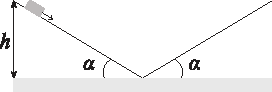
\includegraphics[width=\linewidth]{2008-lahg-02-yl}
	\end{center}
\end{wrapfigure}
Kelguga lastakse alla $h = \SI{10}{m}$ kõrgusest $\alpha = \ang{30}$ kaldenurgaga orunõlvast. Kui kõrgele tõuseb kelk saadud hooga mööda sama suure kaldenurgaga vastasnõlva, kui hõõrdetegur on $\mu = \num{0,1}$? 

\emph{Märkus}: joonis on ligikaudne, languselt tõusule üleminek on tegelikult sujuv ja põrkega seotud kiirusekadu seal ei toimu.

\hint
Kehtib energia jäävuse seadus. Koguenergiate vahe alg- ja lõppseisu vahel kulus hõõrdejõu ületamiseks vajalikuks tööks mõlemal mäenõlval.

\solu
\begin{wrapfigure}[7]{r}{0.3\textwidth}
	\begin{center}
		\vspace{-25pt}
		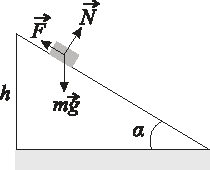
\includegraphics[width=0.95\linewidth]{2008-lahg-02-lah}
	\end{center}
\end{wrapfigure}
Kehtib energia jäävuse seadus. Algul on kelk kõrgusel $h$ ja omab potentsiaalset energiat $mgh$. See energia kulutatakse hõõrdejõu ületamise tööks mõlemal mäenõlval ja kelgu uueks tõusuks vajaliku potentsiaalse energia peale. Energia jäävust väljendab valem 
\begin{equation} \label{2008-lahg-02:eq1}
mgh= A_1+ A_2+ mgh_2,
\end{equation}
kus $h_2$ on kelgu lõppkõrgus. Hõõrdejõud mõlemal nõlval avaldub kujul $F=\mu N=\mu mg \cos\alpha$. Teepikkus laskumisel on $s_1= h/ \sin\alpha$ ning tõusul $s_2= h_2/ \sin\alpha$. Seega tehtud töö hõõdejõu ületamiseks on
\[
A_1= F s_1=\mu mgh/\tan\alpha
\]
ja
\[
A_2= F s_2=\mu mgh_2/\tan\alpha.
\]
Asendades saadud seosed valemisse (\ref{2008-lahg-02:eq1}) saame
\[
h_2= \frac{1 - \mu/\tan\alpha}{1 + \mu/\tan\alpha}h \approx \SI{7}{m}.
\]
\probend